\subsection{Sequential Model}

During the process of optimizing our Sequential model for our NLP (Natural Language Processing) problem, we aimed to enhance the performance by addressing the intricacies of text data. The primary challenge was to capture the complex patterns and contextual relationships within the text to accurately classify emotions. \autocite{sequential-model}

We implemented a Sequential model using Keras to address these challenges. The model architecture was designed to effectively capture the nuances within the text data:

\begin{itemize}
    \item \textbf{Input Layer}: The input layer consists of 2000 features, derived from TF-IDF vectorization, capturing the most significant unigrams and bigrams.
    \item \textbf{Hidden Layers}:
    \begin{itemize}
        \item The first dense layer includes 512 units with ReLU activation and a dropout rate of 0.5 to mitigate overfitting.
        \item The second dense layer comprises 256 units, also with ReLU activation and a dropout rate of 0.5.
        \item The third dense layer has 128 units with ReLU activation and a 0.5 dropout rate.
    \end{itemize}
    \item \textbf{Output Layer}: The final layer consists of six units, corresponding to the six emotion categories (sadness, joy, love, anger, fear, surprise), with softmax activation to output probability distributions.
\end{itemize}

The model was compiled using the Adam optimizer with a learning rate of 0.001 and categorical cross-entropy loss. Accuracy was used as the evaluation metric.


\subsubsection{Evaluation and Results}

After training, the model was evaluated on the test set, achieving an accuracy of 0.89. The classification report indicated the model's precision, recall, and F1-score across different emotion categories, demonstrating the model's effectiveness.

\begin{figure}[H]
    \centering
    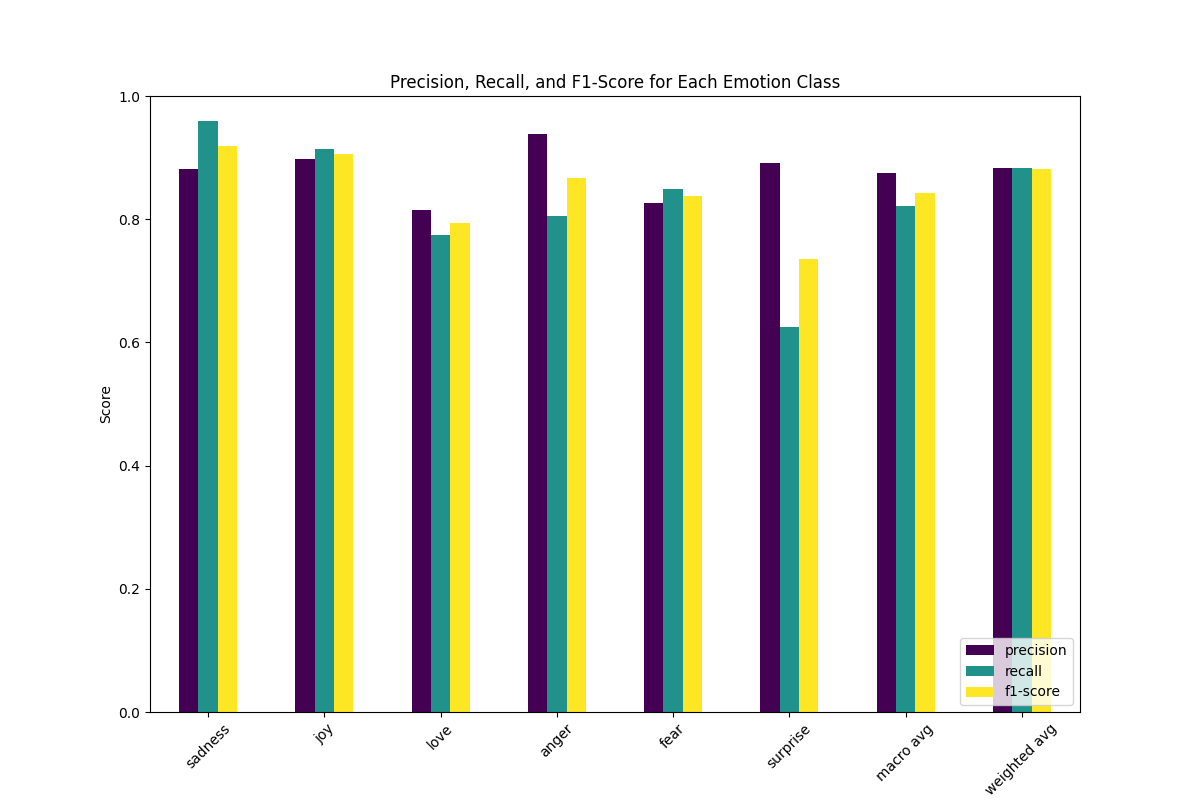
\includegraphics[width=1\columnwidth]{images/Classification_report_model4.png}
    \caption{Precision, Recall, and F1-Score for Each Emotion Class. The model shows strong performance across these metrics, with most scores above 0.8.}
    \label{fig:sequential_model_performance}
\end{figure}
